\documentclass{beamer}
\usetheme{Madrid}
\beamertemplatenavigationsymbolsempty
\usepackage{graphicx}
\usepackage{pgf-soroban}
\usepackage{amsfonts}
\usepackage{amsmath}
\usepackage{xcolor}
\usepackage{tikz}
\usetikzlibrary{shapes.geometric,calc,decorations.text}
\usepackage{stmaryrd}
\usepackage{mathtools}
\usepackage{dsfont}
\usepackage{bussproofs}
\usepackage{hyperref}
\usepackage{fontspec}
\setmonofont{JetBrains Mono}[
    Contextuals = Alternate,
    Ligatures = TeX,
]
\usepackage{listings}
\lstset{
    basicstyle = \ttfamily,
    columns = flexible,
}
\makeatletter
\renewcommand*\verbatim@nolig@list{}
\makeatother
\usepackage{amssymb}
\usepackage{pmboxdraw}

\lstdefinelanguage{Kotlin}{
    basicstyle = \footnotesize\ttfamily,
    comment=[l]{//},
    commentstyle={\color{gray}\ttfamily},
    emph={delegate, filter, lazy, println, return@, K, E},
    emphstyle={\color{red}},
    identifierstyle=\color{black},
    keywords={abstract, actual, as, as?, break, by, class, companion, continue, data, do, dynamic, else, enum, expect, false, final, for, fun, get, if, import, in, interface, internal, is, null, object, operator, override, package, private, public, return, sealed, set, super, suspend, this, throw, true, try, typealias, tailrec, val, var, vararg, when, where, while},
    keywordstyle={\color{blue}\bfseries},
    morecomment=[s]{/*}{*/},
    morestring=[b]",
    morestring=[s]{"""*}{*"""},
    ndkeywords={@Deprecated, @JvmField, @JvmName, @JvmOverloads, @JvmStatic, @JvmSynthetic, Array, Byte, Double, Float, Int, Integer, Iterable, Long, Runnable, Short, String, Bool},
    ndkeywordstyle={\color{orange}\bfseries},
    sensitive=true,
    stringstyle={\color{green}\ttfamily},
    showstringspaces=false,
    escapechar=@
}

\title[Array Programming on $GF(2^n)$]{Probabilistic Array Programming on Galois Fields}
\author[Considine, Guo, Si]{Breandan Considine, Jin Guo, Xujie Si}
\institute[McGill]{
    McGill University, Mila IQIA\\
    \medskip
    \textit{breandan.considine@mail.mcgill.ca}
}
\date{\today}

\begin{document}
    \begin{frame}
        \titlepage
    \end{frame}

    \begin{frame}
        \frametitle{Overview}
        \tableofcontents
    \end{frame}

    \section{Algebraic Parsing}\label{sec:algebraic-parsing}

    %------------------------------------------------------------------------------------------------

    \begin{frame}
        \frametitle{Recap: Context Free Grammars}
        Suppose we have a context free grammar (CFG) $G = \langle V, \Sigma, P, S\rangle$ where $V$ is the set of nonterminals, $\Sigma$ is the terminals, $P: V\times (V \cup \Sigma)^+$ are the productions, $S\in V$ is the start symbol and $+$ is the Kleene plus.\newline\\
        %
        For example, consider the grammar $\underline{S \rightarrow S S \mid ( S ) \mid ()}$. This represents the language of balanced parentheses, e.g. $(), ()(), (()), ()(()), (()()), (())()\ldots$\newline\\
        %
        Every CFG has a normal form $P^*: V \times (V^2 \mid \Sigma)$, i.e., every production can be refactored into either $v_0 \rightarrow v_1 v_2$ or $v_0 \rightarrow \sigma$, where $v_{0\ldots2}: V$ and $\sigma: \Sigma$, e.g., $\underline{S \rightarrow S S \mid ( S ) \mid ()}\Leftrightarrow^*\underline{S\rightarrow XR \mid SS \mid LR, L \rightarrow (, R \rightarrow ), X\rightarrow LS}$

        \begin{center}
        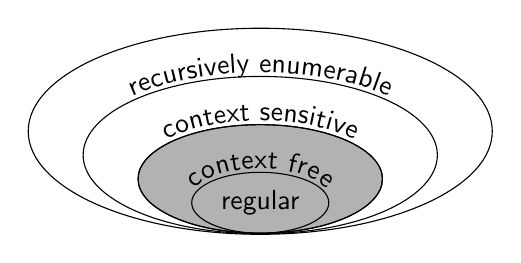
\begin{tikzpicture}[font=\sffamily,breathe dist/.initial=4ex]
            \foreach \X [count=\Y,remember=\Y as \LastY] in
                {regular,context free}
                {\ifnum\Y=1
            \node[ellipse,draw,outer sep=0pt] (F-\Y) {\X};
            \else
            \path[decoration={text along path,
            text={|\sffamily|\X},text align=center,raise=0.3ex},decorate]
        let \p1=($(F-\LastY.north)-(F-\LastY.west)$)
            in (F-\LastY.west) arc(180:0:\x1 and \y1);
            \path let \p1=($([yshift=\pgfkeysvalueof{/tikz/breathe dist}]F-\LastY.north)
            -(F-\LastY.south)$),
            \p2=($(F-1.east)-(F-1.west)$),\p3=($(F-1.north)-(F-1.south)$)
            in ($([yshift=\pgfkeysvalueof{/tikz/breathe dist}]F-\LastY.north)!0.5!(F-\LastY.south)$)
            node[minimum height=\y1,minimum width={\y1*\x2/\y3},
            draw,ellipse,inner sep=0pt, fill=black!30!white] (F-\Y){};
            \fi
            }
            \foreach \X [count=\Y,remember=\Y as \LastY] in
                {regular,context free,context sensitive,recursively enumerable}
                {\ifnum\Y=1
            \node[ellipse,draw,outer sep=0pt] (F-\Y) {\X};
            \else
            \path[decoration={text along path,
            text={|\sffamily|\X},text align=center,raise=0.3ex},decorate]
        let \p1=($(F-\LastY.north)-(F-\LastY.west)$)
            in (F-\LastY.west) arc(180:0:\x1 and \y1);
            \path let \p1=($([yshift=\pgfkeysvalueof{/tikz/breathe dist}]F-\LastY.north)
            -(F-\LastY.south)$),
            \p2=($(F-1.east)-(F-1.west)$),\p3=($(F-1.north)-(F-1.south)$)
            in ($([yshift=\pgfkeysvalueof{/tikz/breathe dist}]F-\LastY.north)!0.5!(F-\LastY.south)$)
            node[minimum height=\y1,minimum width={\y1*\x2/\y3},
            draw,ellipse,inner sep=0pt] (F-\Y){};
            \fi}
        \end{tikzpicture}
        \end{center}
    \end{frame}


    \begin{frame}
        \frametitle{Algebraic parsing, distilled}
        Given a CFG $\mathcal{G} \coloneqq \langle V, \Sigma, P, S\rangle$ in Chomsky Normal Form, we can construct a recognizer $R_\mathcal{G}: \Sigma^n \rightarrow \mathbb{B}$ for strings $\sigma: \Sigma^n$ as follows. Let $\mathcal P(V)$ be our domain, $0$ be $\varnothing$, $\oplus$ be $\cup$, and $\otimes$ be defined as:

        \vspace{-7pt}
        \[
            a \otimes b \coloneqq \{C \mid \langle A, B\rangle \in a \times b, (C\rightarrow AB) \in P\}
        \]

        \noindent We initialize $\mathbf{M}^0_{r,c}(\mathcal{G}, \sigma) \coloneqq \{V \mid c = r + 1, (V \rightarrow \sigma_r) \in P\}$ and search for a matrix $\mathbf{M}^*$ via fixpoint iteration,

        \vspace{-5}
        \[
            \mathbf{M}^* = \begin{pmatrix}
                               \varnothing & \{V\}_{\sigma_1} & \ldots & \ldots & \mathcal{T} \\
                               \varnothing & \varnothing & \{V\}_{\sigma_2} & \ldots & \ldots \\
                               \varnothing & \varnothing & \varnothing & \{V\}_{\sigma_3} & \ldots \\
                               \varnothing & \varnothing & \varnothing & \varnothing & \{V\}_{\sigma_4} \\
                               \varnothing & \varnothing & \varnothing & \varnothing & \varnothing
            \end{pmatrix}
        \]

        \noindent where $\mathbf{M}^*$ is the least solution to $\mathbf{M} = \mathbf{M} + \mathbf{M}^2$. We can then define the recognizer as $R \coloneqq \mathds{1}_{\mathcal{T}}(S) \iff \mathds{1}_{\mathcal{L}(\mathcal{G})}(\sigma)$.
    \end{frame}

    \begin{frame}[fragile]
        \frametitle{Kotlin implementation: CFG definition}
        \begin{lstlisting}[language=Kotlin, gobble=8, basicstyle=\scriptsize\ttfamily]
        typealias Production = Pair<String, List<String>>
        typealias CFG = Set<Production>
        val Production.LHS: String get() = first
        val Production.RHS: List<String> get() = second
        val CFG.nonterminals: Set<String> by cache { map { it.LHS }.toSet() }
        val CFG.words: Set<String> by cache { nonterminals + flatMap { it.RHS } }
        val CFG.terminals: Set<String> by cache { words - nonterminals }
        // Many-to-many mapping of nonterminals to RHS expansions
        val CFG.bimap: BidirectionalMap by cache { BidirectionalMap(this) }

        fun CFG.makeAlgebra(): Ring<Set<String>> =
          Ring.of(
            // 0 = ∅
            nil = setOf(),
            // x + y = x @\texttt{∪}@ y
            plus = { x, y -> x union y },
            // x · y = { A0 | A1 @\texttt{∈}@ x, A2 @\texttt{∈}@ y, (A0 -> A1 A2) @\texttt{∈}@ P }
            times = { x, y -> join(x, y) }
          )

        fun CFG.join(ls: Set<String>, rs: Set<String>): Set<String> =
          (ls * rs).flatMap { (l, r) -> bimap[listOf(l, r)] }.toSet()
        \end{lstlisting}
    \end{frame}

    \begin{frame}[fragile]
        \frametitle{Kotlin implementation: the recognizer}
        \begin{lstlisting}[language=Kotlin, gobble=8, basicstyle=\scriptsize\ttfamily]
        // Adds singleton NTs to superdiagonal: σ_i = { A | (A -> w[i]) ∈ P }
        fun CFG.initialMatrix(str: List<String>): Matrix<Set<String>> =
          Matrix(makeAlgebra(), str.size + 1) { i, j ->
            if (i + 1 != j) emptySet() else bimap[listOf(str[j - 1])].toSet()
          }

        tailrec fun <T: Matrix<S>, S> T.seekFixpoint(op: (T) -> T): T {
          val next = op(this)
          return if (this == next) next else next.seekFixpoint(op)
        }

        fun CFG.isValid(str: String): Boolean =
          tokenize(str).let { START_SYMBOL in parse(it).map { it.root } }

        // Since matrix is strictly UT, must converge in < |tokens| steps
        fun CFG.parse(tokens: List<String>): Set<String> =
            initialMatrix(tokens).seekFixpoint { it + it * it }.first()[0]
        \end{lstlisting}
    \end{frame}


    \begin{frame}
        \frametitle{A few observations on algebraic parsing}
        \begin{itemize}
            \item The matrix $\mathbf M^*$ is strictly upper triangular, i.e., nilpotent of degree $n$
            \item The $\otimes$ operator is (sadly) \textit{not} associative TODO: give example
            \item Recognizer easily translated into a parser by storing backpointers
            \item Built-in error recovery: nonempty submatrices = parsable fragments
            \item \texttt{seekFixpoint \{ it + it * it \}} is sufficient but unnecessary
            \item What if there were some way to solve for $\mathbf{M = M + M}^2$ directly?
            \item Can be lowered onto a Boolean tensor $\mathbb{B}^{n\times n \times |V|}$ (Valiant, 1975)
            \item Na\"ively, has complexity $\mathcal{O}(n^4)$, can be reduced to $\mathcal{O}(n^\omega)$ (Lee, 1997)
        \end{itemize}
    \end{frame}

    \begin{frame}
        \frametitle{Satisfiability + holes (our contribution!)}
        \begin{itemize}
            \item Binarized CYK parser can be efficiently compiled to a SAT solver
            \item Supports sketch-based synthesis in the string or grammar
            \item We simply encode the characteristic function, i.e. $\mathds{1}_{\subseteq V}: V\rightarrow \mathbb{B}^{|V|}$
            \item $\oplus$ is defined as $\boxplus$ and $\otimes$ is $\boxtimes$, where $\boxplus, \boxtimes: \mathbb{B}^{|V|}\times\mathbb{B}^{|V|} \rightarrow \mathbb{B}^{|V|}$
            \item These operators can be lifted into matrices/tensors in the usual way
            \item In most cases, only a few nonterminals are active at any given time
            \item More sophisticated encodings are known for $\binom{n}{0 \leq k}$ subsets
            \item If density is desired, possible to use the Maculay representation
            \item Set joins are an active topic of research in SQL query optimization
            \item If you know of a more efficient encoding, I want to talk to you!
        \end{itemize}
    \end{frame}

    \begin{frame}
        \frametitle{Abbreviated history of algebraic parsing}
        \begin{itemize}
            \item Cocke–Younger–Kasami (1961) - bottom-up dynamic programming
            \item Brzozowski (1964) - Derivatives of regular expressions
            \item Earley (1968) - top-down dynamic programming (no CNF needed)
            \item Valiant (1975) - realizes Boolean matrix multiplication correspondence
            \item Lee (1997) - Fast CFG Parsing $\Longleftrightarrow$ Fast BMM, formalizes reduction
            \item Might et al. (2011) - Parsing with derivatives (Brzozowski $\Rightarrow$ CFL)
            \item Bakinova, Okhotin et al. (2010) - Formal languages over GF(2)
            \item Bernady \& Jansson (2015) - Certifies Valiant (1975) in Agda
            \item \textbf{Considine (2022) - Encodes Valiant (1975) into SAT + holes}
        \end{itemize}
    \end{frame}

%    \section{IDE Tool}\label{sec:ide}
%
%    \section{Tidyparse tool}\label{sec:tidyparse}

    \section{Typelevel Abacus}

    \begin{frame}
        \frametitle{Abacus arithmetic}
        \begin{itemize}
        \item Computational complexity of arithmetic is notation-dependent(!)
        \item For example, $\pm$ in unary arithmetic is concatenation and decatenation
        \item Multiplication and division by natural powers of the radix is $\mathcal{O}(1)$.
        \item We can describe the abacus as a kind of abstract rewriting system.
        \end{itemize}
        \ladj{0.25}
        \begin{prooftree}
            \AxiomC{
                \tikz \fill [white] (0,0) rectangle (1,2);
            }
            \UnaryInfC{
                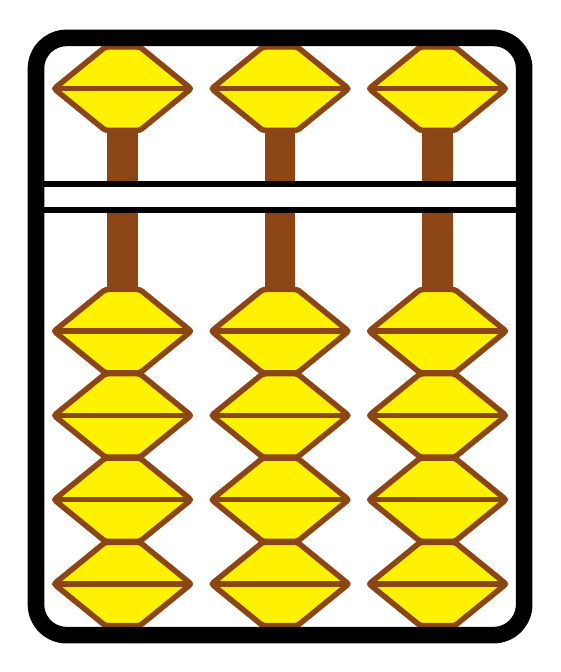
\begin{tikzpicture}
                    \tige{1}{0}{0}
                    \tige{2}{0}{0}
                    \tige{3}{0}{0}
                    \cadre{3}
                \end{tikzpicture}
            }
            \DisplayProof
            \hskip 1em
            \AxiomC{
                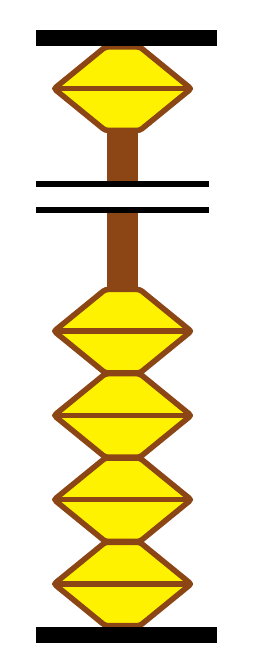
\begin{tikzpicture}
                    \tige{1}{0}{0}
                    \barres{1}
                \end{tikzpicture}$_n+10^n$
            }
            \UnaryInfC{
                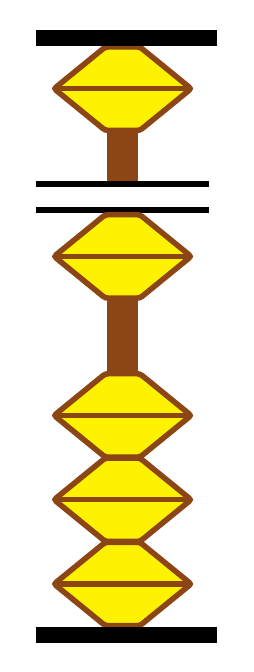
\begin{tikzpicture}
                    \tige{1}{1}{0}
                    \barres{1}
                \end{tikzpicture}$_n\phantom{n+0^n}$
            }
            \DisplayProof
            \hskip 1em
            \AxiomC{
                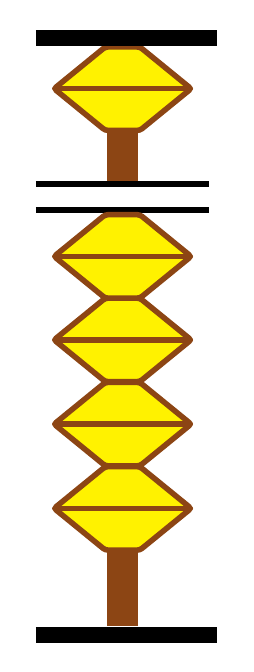
\begin{tikzpicture}
                    \tige{1}{4}{0}
                    \barres{1}
                \end{tikzpicture}$_n+10^n$
            }
            \UnaryInfC{
                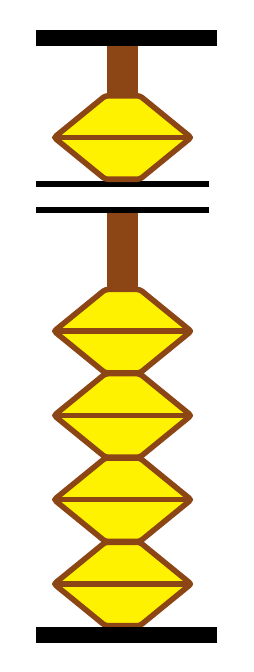
\begin{tikzpicture}
                    \tige{1}{5}{0}
                    \barres{1}
                \end{tikzpicture}$_n\phantom{n+0^n}$
            }
            \DisplayProof
            \hskip 1em
            \AxiomC{
                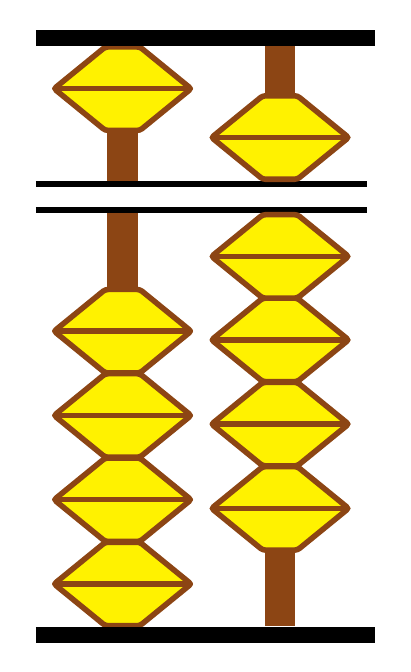
\begin{tikzpicture}
                    \tige{1}{0}{0}
                    \barres{1}
                    \tige[2]{1}{9}{0}
                    \barres[2]{1}
                \end{tikzpicture}$_n+10^n$
            }
            \UnaryInfC{
                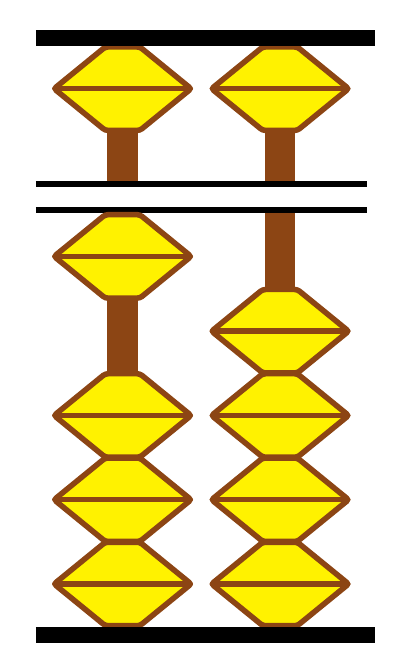
\begin{tikzpicture}
                \tige{1}{1}{0}
                \barres{1}
                \tige[2]{1}{0}{0}
                \barres[2]{1}
                \end{tikzpicture}$_n\phantom{n+0^n}$
            }
        \end{prooftree}
    \end{frame}

    \begin{frame}[fragile]
        \frametitle{Abacus dependent types}
        \begin{lstlisting}[language=Kotlin, gobble=7]
        sealed class B<X, P : B<X, P>>(open val x: X? = null) {
          val T: T<P> get() = T(this as P)
          val F: F<P> get() = F(this as P)
        }

        class U(val i: Int) : B<Any, U>() // Checked at runtime

        object Ø: B<Ø, Ø>(null)           // Nothing

        class T<X>(override val x: X = Ø as X) : B<X, T<X>>(x)
          { companion object: T<Ø>(Ø) }

        class F<X>(override val x: X = Ø as X) : B<X, F<X>>(x)
          { companion object: F<Ø>(Ø) }

        val b0: F<Ø> = F
        val b1: T<Ø> = T
        val b2: F<T<Ø>> = T.F
        val b3: T<T<Ø>> = T.T
        val b4: F<F<T<Ø>>> = T.F.F
        \end{lstlisting}
    \end{frame}

    \begin{frame}[fragile]
        \frametitle{Abacus dependent types up to $2^n-1$ where $n=4$}
        \begin{lstlisting}[language=Kotlin, gobble=7]
        typealias B_0<K> = F<K>
        typealias B_1<K> = T<K>
        typealias B_2<K> = F<T<K>>
        typealias B_3<K> = T<T<K>>
        typealias B_4<K> = F<F<T<K>>>
        typealias B_7<K> = T<T<T<K>>>
        typealias B_8<K> = F<F<F<T<K>>>>

        operator fun Ø.plus(t: T<Ø>) = b1
        operator fun B_0<Ø>.plus(t: T<Ø>) = b1
        operator fun B_1<Ø>.plus(t: T<Ø>): B_2<Ø> = F(x + b1)
        operator fun B_3<Ø>.plus(t: T<Ø>): B_4<Ø> = F(x + b1)
        operator fun B_7<Ø>.plus(t: T<Ø>): B_8<Ø> = F(x + b1)

        operator fun <K: B<*, *>> B_0<K>.plus(t: T<Ø>) = T(x)
        operator fun <K: B<*, *>> B_1<F<K>>.plus(t: T<Ø>) = F(x + b1)
        operator fun <K: B<*, *>> B_3<F<K>>.plus(t: T<Ø>) = F(x + b1)
        operator fun <K: B<*, *>> B_7<F<K>>.plus(t: T<Ø>) = F(x + b1)
        \end{lstlisting}
    \end{frame}

    \begin{frame}[fragile]
        \frametitle{Abacus dependent types: birds eye view}
        \begin{tiny}
        \begin{verbatim}
            i │  0  1  …  k-1  k  │  k+1  k+2  …  k+c  │  k+c+1  …  k+c+k
           ───┼───────────────────┼────────────────────┼───────────────────┐ ┐
            0 │                   │                    │                __/  │
            1 │                   │                    │             __/XXX  │
            … │       i ± i       │        k ± i       │          __/XXXXXX  ├ ┐
          k-1 │                   │                    │      ___/XXXXXXXXX  │ │
            k │                   │                    │  ___╱XXXXXXXXXXXXX  │ │
          ────┼───────────────────┼────────────────────┴─┘XXXXXXXXXXXXXXXXX  ┘ │
          k+1 │                   │XXXXXXXXXXXXXXXXXXXXXXXXXXXXXXXXXXXXXXXX    │
          k+2 │                   │XXXXXXXXXXXXXXXXXXXXXXXXXXXXXXXXXXXXXXXX    │
            … │       i ± k       │XXXXXXXXXXXXXXXXXXXXXXXXXXXXXXXXXXXXXXXX    │
            … │                   │XXXXXXXXXXXXXXXXXXXXXXXXXXXXXXXXXXXXXXXX    │
          k+c │                   │XXXXXXXXXXXX                XXXXXXXXXXXX    │
         ─────┼───────────────────┤XXXXXXXXXXXX    Run-time    XXXXXXXXXXXX    │
        k+c+1 │               ___/XXXXXXXXXXXXX  type checked  XXXXXXXXXXXX    │
            … │           ___/XXXXXXXXXXXXXXXXX                XXXXXXXXXXXX    │
            … │       ___/XXXXXXXXXXXXXXXXXXXXXXXXXXXXXXXXXXXXXXXXXXXXXXXXX    │
            … │   ___/XXXXXXXXXXXXXXXXXXXXXXXXXXXXXXXXXXXXXXXXXXXXXXXXXXXXX    │
        k+c+k │__/XXXXXXXXXXXXXXXXXXXXXXXXXXXXXXXXXXXXXXXXXXXXXXXXXXXXXXXXX    │

              └─────────┬─────────┘                               Compile-time
                        └─────────────────────────────────────    type checked
        \end{verbatim}
        \end{tiny}
    \end{frame}

    \begin{frame}
        \frametitle{Annotated history of typed EDSLs}
        \begin{itemize}
            \item Canning et al. (1989) invents F-Bounded Polymorphism
            \item Hinze (2003) - Discovers Phantom types (useful for type-safe builders)
            \item Eder (2011) - Encodes relational algebra into j[ava]OOQ
            \item Grigore (2016) - Java Generics shown to be Turing Complete
            \item Erdős (2017) - Encodes Boolean logic into Java type system
            \item Nakamaru (2017) - Silverchain: fluent API generator
            \item \textbf{Considine (2019) - Shape-safe matrix multiplication in Kotlin$\nabla$}
            \item Fling (2019) - Fling, A Fluent API parser generator
            \item Roth (2021) - Encodes CFL into Nominal Subtyping with Variance
            \item \textbf{Considine (2021) - Arithmetic in Kotlin via typelevel abacus}
            \item We know how to lower parsing onto types, what about vis versa?
        \end{itemize}
    \end{frame}

    \begin{frame}[fragile]
        \frametitle{Can we lower type checking onto parsing?}
        First, let us consider the untyped version:
        \begin{lstlisting}[language=Kotlin, gobble=5]
        Exp -> 0 | 1 | ... | T | F
        Exp -> Exp Op Exp | if ( Exp ) Exp else Exp
        Op -> and | or | + | *
        \end{lstlisting}
        Now, let us consider the GADT/HOAS version:
        \begin{lstlisting}[language=Kotlin, gobble=5]
        Exp<Bool> -> T | F
        Op<Bool> -> and | or
        Exp<Int> -> 0 | 1 | ... | 9
        Op<Int> -> + | *
        Exp<E> -> Exp<E> Op<E> Exp<E> // Es must match exactly!
        Exp<E> -> if ( Exp<Bool> ) Exp<E> else Exp<E>
        \end{lstlisting}
        We can eliminate context sensitivity by concretizing \lstinline[language=Kotlin]{E -> Bool | Int}:
        \begin{lstlisting}[language=Kotlin, gobble=5]
        Exp<Bool> -> T | F
        Exp<Bool> -> Exp<Bool> or Exp<Bool> | Exp<Bool> and Exp<Bool>
        Exp<Bool> -> if ( Exp<Bool> ) Exp<Bool> else Exp<Bool>
        Exp<Int> -> 0 | 1 | ... | 9
        Exp<Int> -> Exp<Int> + Exp<Int> | Exp<Int> * Exp<Int>
        Exp<Int> -> if ( Exp<Bool> ) Exp<Int> else Exp<Int>
        \end{lstlisting}

    \end{frame}

    \begin{frame}
        \begin{center}
            \Huge{Learn more at: \\~\\
            \href{http://array22.ndan.co}{\color{blue}{http://array22.ndan.co}}}
        \end{center}
    \end{frame}

    \begin{frame}
        \frametitle{Special thanks}
            \begin{center}
                \LARGE{
                    Nghi D. Q. Bui\\
                    Zhixin Xiong\\
                    Jaylene Zhang\\
                    David Yu-Tung Hui\\
                    Fabian Muehlboeck\\
                    Ben Greenman
                }

                
\includegraphics[scale=0.3]{../figures/fpt_logo.png}
                
\includegraphics[scale=0.2]{../figures/mila_logo.png}
            \end{center}
    \end{frame}
\end{document}